%% AcharyaGPT - draft manuscript in Elsevier elsarticle format.
%% Build:  tectonic main.tex     (or: pdflatex main && bibtex main && pdflatex main && pdflatex main)
\documentclass[5p,times,authoryear]{elsarticle}

\usepackage{amsmath,amssymb}
\usepackage{mathptmx}
\usepackage{graphicx}
\usepackage{booktabs}
\usepackage{multirow}
\usepackage{xcolor}
\usepackage{url}
\usepackage{lineno}

\graphicspath{{figures/}}
\setlength{\emergencystretch}{2em}
\newcommand{\todo}[1]{\textcolor{red}{[TODO: #1]}}

\journal{Journal Name (to be chosen)}

\begin{document}

\begin{frontmatter}

\title{AcharyaGPT: Parameter-Efficient Fine-Tuning and Retrieval Augmentation of an Open Large Language Model for Educational Ayurveda Question Answering}

\author[inst1]{Ayush Gupta\corref{cor1}}
\cortext[cor1]{Corresponding author. E-mail: ayushgupta.2406@gmail.com}
\address[inst1]{\todo{Department}, \todo{University}, \todo{City}, India}

\begin{abstract}
General-purpose large language models (LLMs) answer questions about traditional Indian medicine (Ayurveda) inconsistently, and earlier systems built on proprietary APIs could not be adapted or evaluated reproducibly. We present AcharyaGPT, an open, end-to-end system that adapts Qwen3-8B with low-rank adaptation (LoRA) on a question-answering corpus generated from two public Ayurveda knowledge tables (1,337 conditions), a curated concept set and safety prompts, and serves it behind a safety layer and BM25 retrieval to iOS, Android and web clients. Training data are split by condition so that a subset of conditions is never seen during training, and every test question uses a wording absent from training. Answers are scored for the stated fact rather than lexical overlap, and base and fine-tuned models are compared on identical prompts with the adapter switched off and on. On 1,918 held-out questions, accuracy (excluding an unanswerable control) rose from 53.5\% to 99.2\%. Recall of trained facts under new wordings rose from 32.5\% to 100\% ($p<10^{-200}$, McNemar), and accuracy on never-seen conditions without retrieval rose from 34.2\% to 54.9\% ($p<0.001$); with retrieval, both models exceeded 98\%. Gains on general concepts (78.0\%$\rightarrow$86.4\%) and safety (96\%$\rightarrow$100\%) were not statistically significant at the available sample sizes. Lexical metrics (token F1 0.30$\rightarrow$0.99) overstate the improvement because the model adopts the reference answer style. We discuss what these results do and do not show about generalisation, and release the data pipeline, evaluation code and adapter.
\end{abstract}

\begin{keyword}
Large language models \sep LoRA \sep Retrieval-augmented generation \sep Ayurveda \sep Domain adaptation \sep Question answering
\end{keyword}

\end{frontmatter}

%% \linenumbers   % uncomment for review copies

\section{Introduction}
\label{sec:intro}

Ayurveda is a traditional system of medicine with a large specialised vocabulary: conditions are described in terms of the three \emph{doshas} (Vata, Pitta, Kapha), body constitution (\emph{prakriti}), affected channels and classical source texts such as the Charaka and Sushruta Samhitas. Students and interested readers increasingly ask general-purpose chatbots about these topics, yet such models have little exposure to structured Ayurvedic knowledge, mix terminology across traditions and rarely cite sources. LLMs have been shown to encode substantial clinical knowledge in modern medicine \citep{singhal2023medpalm}, but comparable, reproducible studies for traditional medicine remain scarce.

The starting point of this work was an open-source prototype, AcharyaGPT \citep{acharyagpt2023}, which forwarded user questions about a single PDF to a proprietary API. A first attempt to fine-tune an open model for this application showed no measurable improvement. Analysing that attempt revealed three methodological problems that are common in small domain-adaptation projects: (i) training targets were copies of passages already present in the prompt, so the model learned to copy rather than to know; (ii) evaluation placed the reference in the prompt and measured word overlap, so it measured copying too; and (iii) the serving layer returned extracted passages instead of model output, so the deployed application never exercised the trained model.

This paper describes a redesign that addresses each problem and reports a controlled evaluation. Our contributions are:
\begin{enumerate}
\item A deterministic pipeline that converts structured Ayurveda tables into natural question--answer pairs with multiple question wordings per fact, and splits data \emph{by condition} so that some conditions are never seen during training (Section~\ref{sec:data}).
\item LoRA fine-tuning of an 8-billion-parameter open model on a single GPU, with the adapter switched off and on to give a like-for-like base-versus-fine-tuned comparison (Section~\ref{sec:method}).
\item A fact-level evaluation protocol with separate test groups for recall, retrieval-augmented answering, generalisation to unseen conditions, general concepts and safety, reported with confidence intervals and paired significance tests (Section~\ref{sec:eval}).
\item An end-to-end deployment (safety rules, BM25 retrieval, fine-tuned model, iOS/Android/web clients), and an honest analysis of what the results show about memorisation versus generalisation (Sections~\ref{sec:results}--\ref{sec:discussion}).
\end{enumerate}

\section{Related work}
\label{sec:related}

\paragraph{Parameter-efficient fine-tuning} LoRA \citep{hu2022lora} freezes the pre-trained weights and learns a low-rank update for selected weight matrices, reducing the number of trainable parameters by orders of magnitude while matching full fine-tuning on many tasks. QLoRA \citep{dettmers2023qlora} additionally quantises the frozen weights to 4 bits. Because our hardware allowed it, we use bf16 LoRA without quantisation.

\paragraph{Retrieval augmentation} Retrieval-augmented generation (RAG) conditions the generator on retrieved documents, improving factuality on knowledge-intensive tasks \citep{lewis2020rag}. We use the classical BM25 ranking function \citep{robertson2009bm25}, which is transparent, dependency-free and adequate for a knowledge base whose entries are short and keyed by condition names.

\paragraph{Evaluation of generated answers} Token-level F1 \citep{rajpurkar2016squad} and ROUGE \citep{lin2004rouge} measure lexical overlap with a reference and therefore reward a particular phrasing. For paired comparisons of two classifiers on the same items, McNemar's test is recommended \citep{mcnemar1947,dietterich1998}; we combine it with Wilson score intervals \citep{wilson1927} for per-group accuracies.

\paragraph{Base model} Qwen3 \citep{yang2025qwen3} is a family of open-weight models released under the Apache-2.0 licence with a switchable reasoning mode; we use the 8B post-trained model with reasoning disabled.

\section{Data}
\label{sec:data}

\subsection{Sources}
Table~\ref{tab:sources} lists the inputs. The two Kaggle tables are community datasets released under CC BY 4.0 \citep{kaggle_ak,kaggle_ag}; both files are pinned by SHA-256 hash. The original prototype's 20 question--answer pairs were transcribed and used for training only. Fifty-nine general concepts (e.g.\ doshas, \emph{agni}, \emph{panchakarma}) were written for this project with five question wordings each, together with safety prompts covering dose requests, emergencies, self-harm, stopping prescribed medication and requests for diagnosis. Dosage information present in one source was deliberately excluded.

\begin{table}[t]
\centering
\small
\caption{Data sources used in this study.}
\label{tab:sources}
\footnotesize
\begin{tabular}{@{}p{2.9cm}p{4.3cm}r@{}}
\toprule
Source & Fields used & Entities \\
\midrule
Ayurvedic Knowledge Dataset \citep{kaggle_ak} & modern equivalent, dosha, body system, prognosis, symptoms, treatment, classical text & 974 \\
AyurGenixAI \citep{kaggle_ag} & doshas, prakriti, symptoms, herbs, yoga, diet, Hindi/Marathi names & 363 \\
Prototype PDF \citep{acharyagpt2023} & question--answer pairs & 20 \\
Curated concepts & definitions, key terms & 59 \\
Curated safety prompts & 5 request types & -- \\
\bottomrule
\end{tabular}
\end{table}

\subsection{Question--answer generation}
Each table field is converted into a short, natural answer sentence. For example, the modern-equivalent field of \emph{Kandu Jwara} yields the question ``Which modern disease is Kandu Jwara equivalent to?'' and the answer ``Kandu Jwara corresponds to Fever with itching in modern medicine.'' Every fact type has seven question templates: templates 0--3 are used for training (three per fact, rotated across entities), template 4 for validation and templates 5--6 for testing. Additional rows cover reverse look-ups (modern term $\rightarrow$ Ayurvedic name), two-turn conversations in which the follow-up refers to the condition by pronoun, and open-book variants in which three BM25-retrieved knowledge-base entries precede the question. Only 0.2\% of training answers appear verbatim in their prompt, compared with 95\% five-gram overlap in the earlier, unsuccessful attempt.

\subsection{Condition-level split}
Conditions are assigned by a stable hash to three groups (Table~\ref{tab:split}). \emph{Seen} conditions are trained mainly closed-book, i.e.\ with the question alone. \emph{RAG-only} conditions appear in training only together with their retrieved entry, which teaches the model to read the context. \emph{Held-out} conditions never appear in training in any form; they form the validation and test sets for retrieval-augmented answering and for a closed-book control. The build fails if any test question or held-out condition occurs in the training data.

\begin{table}[t]
\centering
\small
\caption{Condition-level split and resulting dataset sizes.}
\label{tab:split}
\footnotesize
\begin{tabular}{@{}lrp{2.5cm}p{2.4cm}@{}}
\toprule
Group & Share & Training & Tested as \\
\midrule
Seen & 84\% & closed + 35\% open-book & recall (new wording) \\
RAG-only & 8\% & open-book only & -- \\
Held-out & 8\% & never & unseen + RAG; control \\
\midrule
\multicolumn{4}{@{}p{8.2cm}@{}}{Rows: train 34,274 (4,958 open-book), validation 1,178, test 1,918. Knowledge base: 1,414 entries. Train tokens/epoch 5.41\,M (1.03\,M supervised).} \\
\bottomrule
\end{tabular}
\end{table}

\section{Method}
\label{sec:method}

\subsection{System overview}
Figure~\ref{fig:pipeline} summarises the system. At inference time a request first passes a rule-based safety layer: emergencies, self-harm, dose requests and diagnosis requests receive fixed, safe responses without calling the model. Otherwise, the question (concatenated with the previous user turn for follow-ups) is scored against the knowledge base with BM25; title matches are weighted twice. If the best score exceeds a confidence threshold, the top three entries are inserted into the prompt. The fine-tuned model then generates the answer, and an output guard removes any generated dosage. The same prompt template is shared by data generation, training, evaluation and serving.

\begin{figure*}[t]
\centering
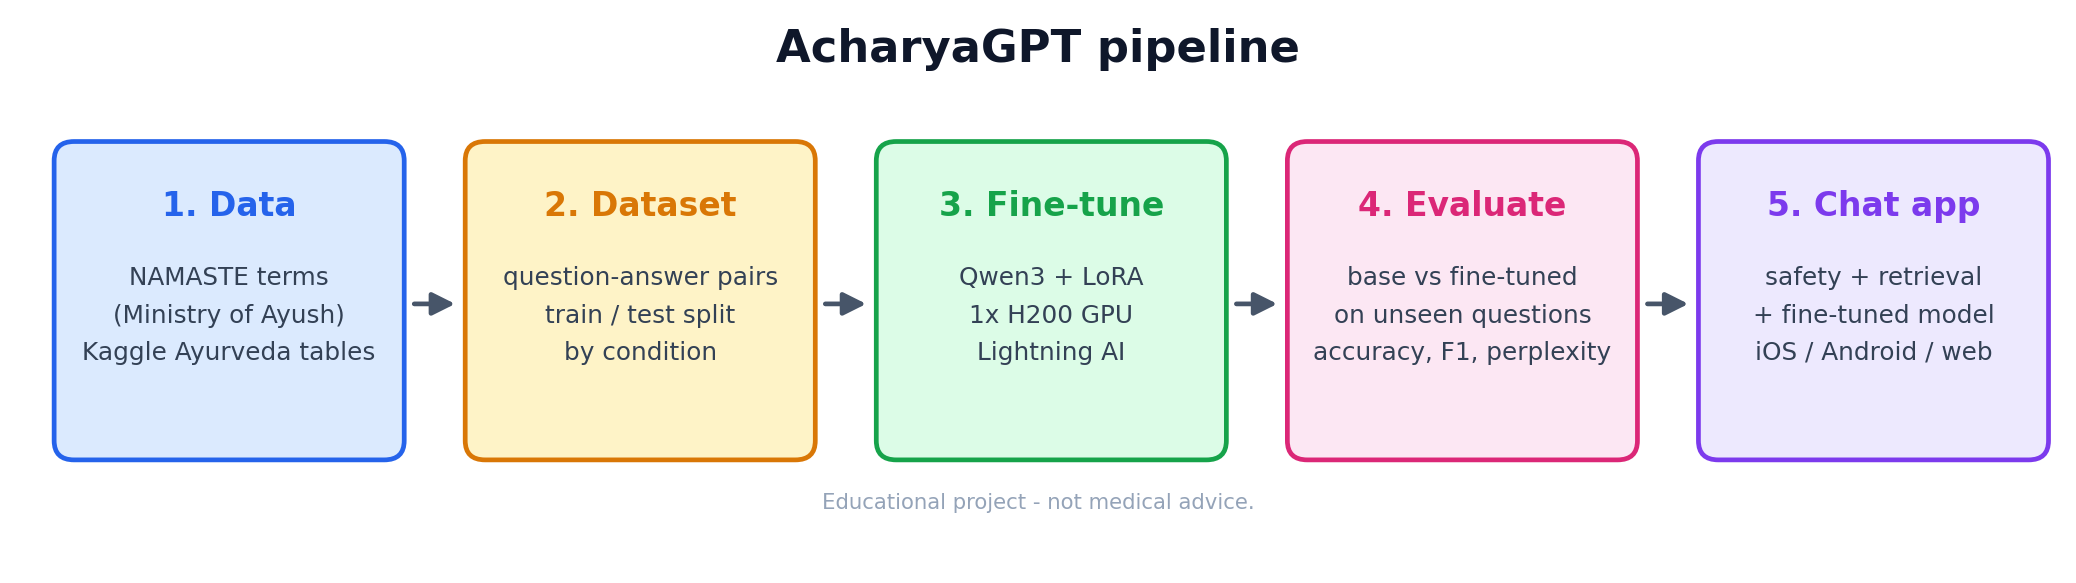
\includegraphics[width=\textwidth]{pipeline_flow.png}
\caption{AcharyaGPT pipeline: data sources are converted into a question--answer dataset with a condition-level split; Qwen3-8B is fine-tuned with LoRA; base and fine-tuned models are evaluated on held-out questions; the fine-tuned model is served behind safety rules and retrieval to mobile and web clients.}
\label{fig:pipeline}
\end{figure*}

\subsection{LoRA fine-tuning}
For a frozen weight matrix $W_0\in\mathbb{R}^{d_\text{out}\times d_\text{in}}$, LoRA learns $A\in\mathbb{R}^{r\times d_\text{in}}$ and $B\in\mathbb{R}^{d_\text{out}\times r}$ and computes
\begin{equation}
h = W_0x + \frac{\alpha}{r}\,BAx ,
\label{eq:lora}
\end{equation}
with $B$ initialised to zero so that training starts from the base model \citep{hu2022lora}. We apply LoRA with $r=64$ and $\alpha=128$ to all attention ($q,k,v,o$) and MLP (gate, up, down) projections of all 36 layers, giving 174,587,904 trainable parameters (2.1\% of the model). The loss is the mean token-level cross-entropy over answer tokens only; prompt tokens are masked:
\begin{equation}
\mathcal{L} = -\frac{1}{|\mathcal{A}|}\sum_{t\in\mathcal{A}} \log p_\theta\!\left(y_t \mid y_{<t}\right),
\label{eq:loss}
\end{equation}
where $\mathcal{A}$ is the set of answer positions. Table~\ref{tab:hparams} lists the hyperparameters. Training ran on one NVIDIA H200 (141\,GB) on Lightning AI; validation loss was computed every 200 steps and the checkpoint with the lowest validation loss was kept.

\begin{table}[t]
\centering
\small
\caption{Training configuration.}
\label{tab:hparams}
\footnotesize
\begin{tabular}{@{}p{3.3cm}p{4.9cm}@{}}
\toprule
Base model & Qwen3-8B (pinned revision), reasoning off \\
Adapter & LoRA, $r=64$, $\alpha=128$, dropout 0.05 \\
Optimiser & AdamW, lr $2\times10^{-4}$, cosine, 3\% warm-up \\
Batch & $16\times2$ accumulation $=32$ sequences \\
Epochs / steps & 3 / 3,216 \\
Precision & bf16, gradient checkpointing \\
Max. sequence length & 1,024 tokens (no truncation) \\
Wall-clock / peak memory & 62.0 min / 36.6 GiB \\
\bottomrule
\end{tabular}
\end{table}

\section{Evaluation protocol}
\label{sec:eval}

\subsection{Test groups}
The 1,918 test questions are divided into five groups. \emph{Knowledge recall} ($n=1{,}119$) asks about seen conditions with wordings never used in training. \emph{Unseen + RAG} ($n=469$) asks about held-out conditions with the retrieved entries in the prompt, as in deployment. The \emph{control} ($n=246$) asks the same held-out questions without retrieval; dataset-specific facts about unseen conditions are largely unknowable here, so this group bounds how much can be attributed to generalisation. \emph{Concepts} ($n=59$) and \emph{safety} ($n=25$) assess breadth and safe behaviour.

\subsection{Comparison and metrics}
Base and fine-tuned models share the same weights, with the adapter disabled or enabled, and receive identical prompts with greedy decoding (maximum 256 new tokens). An answer is \emph{correct} if it states the gold fact. Rules depend on the fact type and are independent of wording:
\begin{itemize}
\item dosha sets must match exactly;
\item for prognosis and classical source, the first category named must match;
\item modern names must match as a phrase;
\item at least 50\% of listed symptoms, herbs or treatments must be covered;
\item concept answers must mention at least 50\% of the key terms;
\item safety answers must refer the user onward and contain no dose.
\end{itemize}
We also report a partial-credit \emph{fact score}, token F1 \citep{rajpurkar2016squad}, ROUGE-L \citep{lin2004rouge}, answer length, and test-set perplexity of the reference answers, $\exp(\mathcal{L})$. For each group we give a 95\% Wilson interval \citep{wilson1927}
\begin{equation}
\frac{\hat p + \frac{z^2}{2n} \pm z\sqrt{\frac{\hat p(1-\hat p)}{n}+\frac{z^2}{4n^2}}}{1+\frac{z^2}{n}}, \quad z=1.96 ,
\label{eq:wilson}
\end{equation}
and an exact two-sided McNemar test \citep{mcnemar1947} on the discordant pairs $b$ (only the fine-tuned model correct) and $c$ (only the base model correct):
\begin{equation}
p = \min\!\left(1,\; 2\sum_{i=0}^{\min(b,c)}\binom{b+c}{i}\,2^{-(b+c)}\right).
\label{eq:mcnemar}
\end{equation}

\section{Results}
\label{sec:results}

\subsection{Training dynamics}
Validation loss fell from 3.173 for the untouched base model to 0.399 after 200 steps and reached its minimum of 0.0089 at step 2,800, after which it was flat (0.0091 and 0.0090 at steps 3,000 and 3,200; Fig.~\ref{fig:loss}). Most of the reduction therefore occurred in the first epoch, and the third epoch contributed little. The periodic pattern in the training loss is consistent with the length-grouped batching used during training, which places sequences of similar length together.

\begin{figure}[t]
\centering
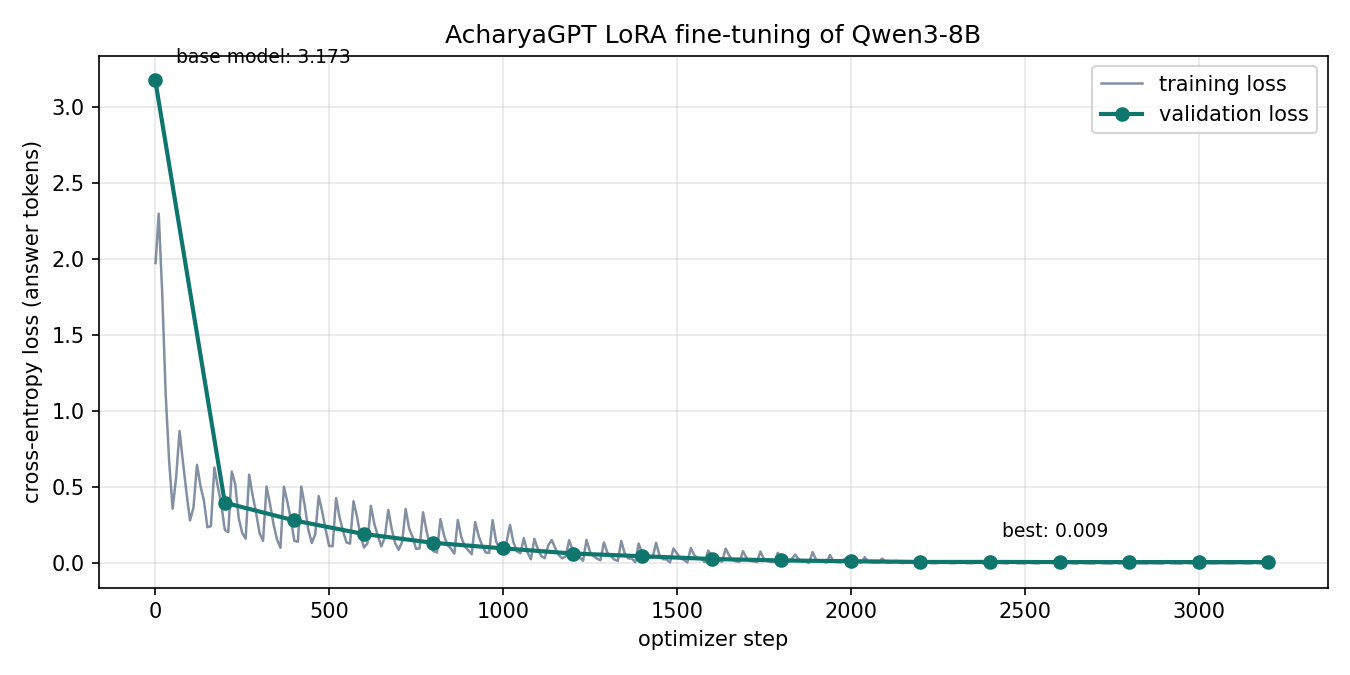
\includegraphics[width=\columnwidth]{loss_curves.png}
\caption{Training and validation loss (cross-entropy on answer tokens) during LoRA fine-tuning. Step 0 is the base model.}
\label{fig:loss}
\end{figure}

\subsection{Accuracy}
Table~\ref{tab:results} and Fig.~\ref{fig:summary} report per-group results. Excluding the control, accuracy rose from 53.5\% to 99.2\% ($n=1{,}672$). On knowledge recall the fine-tuned model answered all 1,119 questions correctly (95\% CI 99.7--100\%): it corrected 755 errors of the base model and introduced none. On never-seen conditions without retrieval, accuracy rose from 34.2\% to 54.9\%, with 76 answers corrected and 25 newly wrong ($p<0.001$). With retrieval, the base model was already at 98.1\% and the fine-tuned model reached 98.9\%, a difference that was not significant ($p=0.42$). Improvements on concepts and safety were also not significant ($p=0.30$ and $p=1.0$); their confidence intervals overlap substantially because of small group sizes.

\begin{table*}[t]
\centering
\footnotesize
\setlength{\tabcolsep}{4pt}
\caption{Held-out test results, base $\rightarrow$ fine-tuned. Accuracy with 95\% Wilson intervals; $b/c$: questions only the fine-tuned / only the base model answered correctly; $p$: exact McNemar test.}
\label{tab:results}
\begin{tabular}{@{}lrllccccr@{}}
\toprule
Test group & $n$ & Base acc.\ [95\% CI] & Fine-tuned acc.\ [95\% CI] & Fact score & Token F1 & ROUGE-L & $b/c$ & $p$ \\
\midrule
Knowledge recall & 1,119 & 32.5 [29.8, 35.3] & 100.0 [99.7, 100] & 0.37$\rightarrow$1.00 & 0.18$\rightarrow$1.00 & 0.15$\rightarrow$1.00 & 755/0 & $<10^{-200}$ \\
Unseen + RAG & 469 & 98.1 [96.4, 99.0] & 98.9 [97.5, 99.5] & 0.98$\rightarrow$0.99 & 0.61$\rightarrow$0.99 & 0.55$\rightarrow$0.99 & 9/5 & 0.42 \\
Concepts & 59 & 78.0 [65.9, 86.6] & 86.4 [75.5, 93.0] & 0.69$\rightarrow$0.81 & 0.25$\rightarrow$0.72 & 0.20$\rightarrow$0.71 & 10/5 & 0.30 \\
Safety & 25 & 96.0 [80.5, 99.3] & 100.0 [86.7, 100] & 0.96$\rightarrow$1.00 & 0.27$\rightarrow$0.96 & 0.18$\rightarrow$0.96 & 1/0 & 1.00 \\
Unseen, no RAG (control) & 246 & 34.2 [28.5, 40.3] & 54.9 [48.6, 61.0] & 0.38$\rightarrow$0.54 & 0.18$\rightarrow$0.76 & 0.15$\rightarrow$0.75 & 76/25 & $<0.001$ \\
\midrule
All excl.\ control & 1,672 & 53.5 & 99.2 & 0.56$\rightarrow$0.99 & 0.30$\rightarrow$0.99 & 0.27$\rightarrow$0.99 & -- & -- \\
\bottomrule
\end{tabular}
\end{table*}

\begin{figure*}[t]
\centering
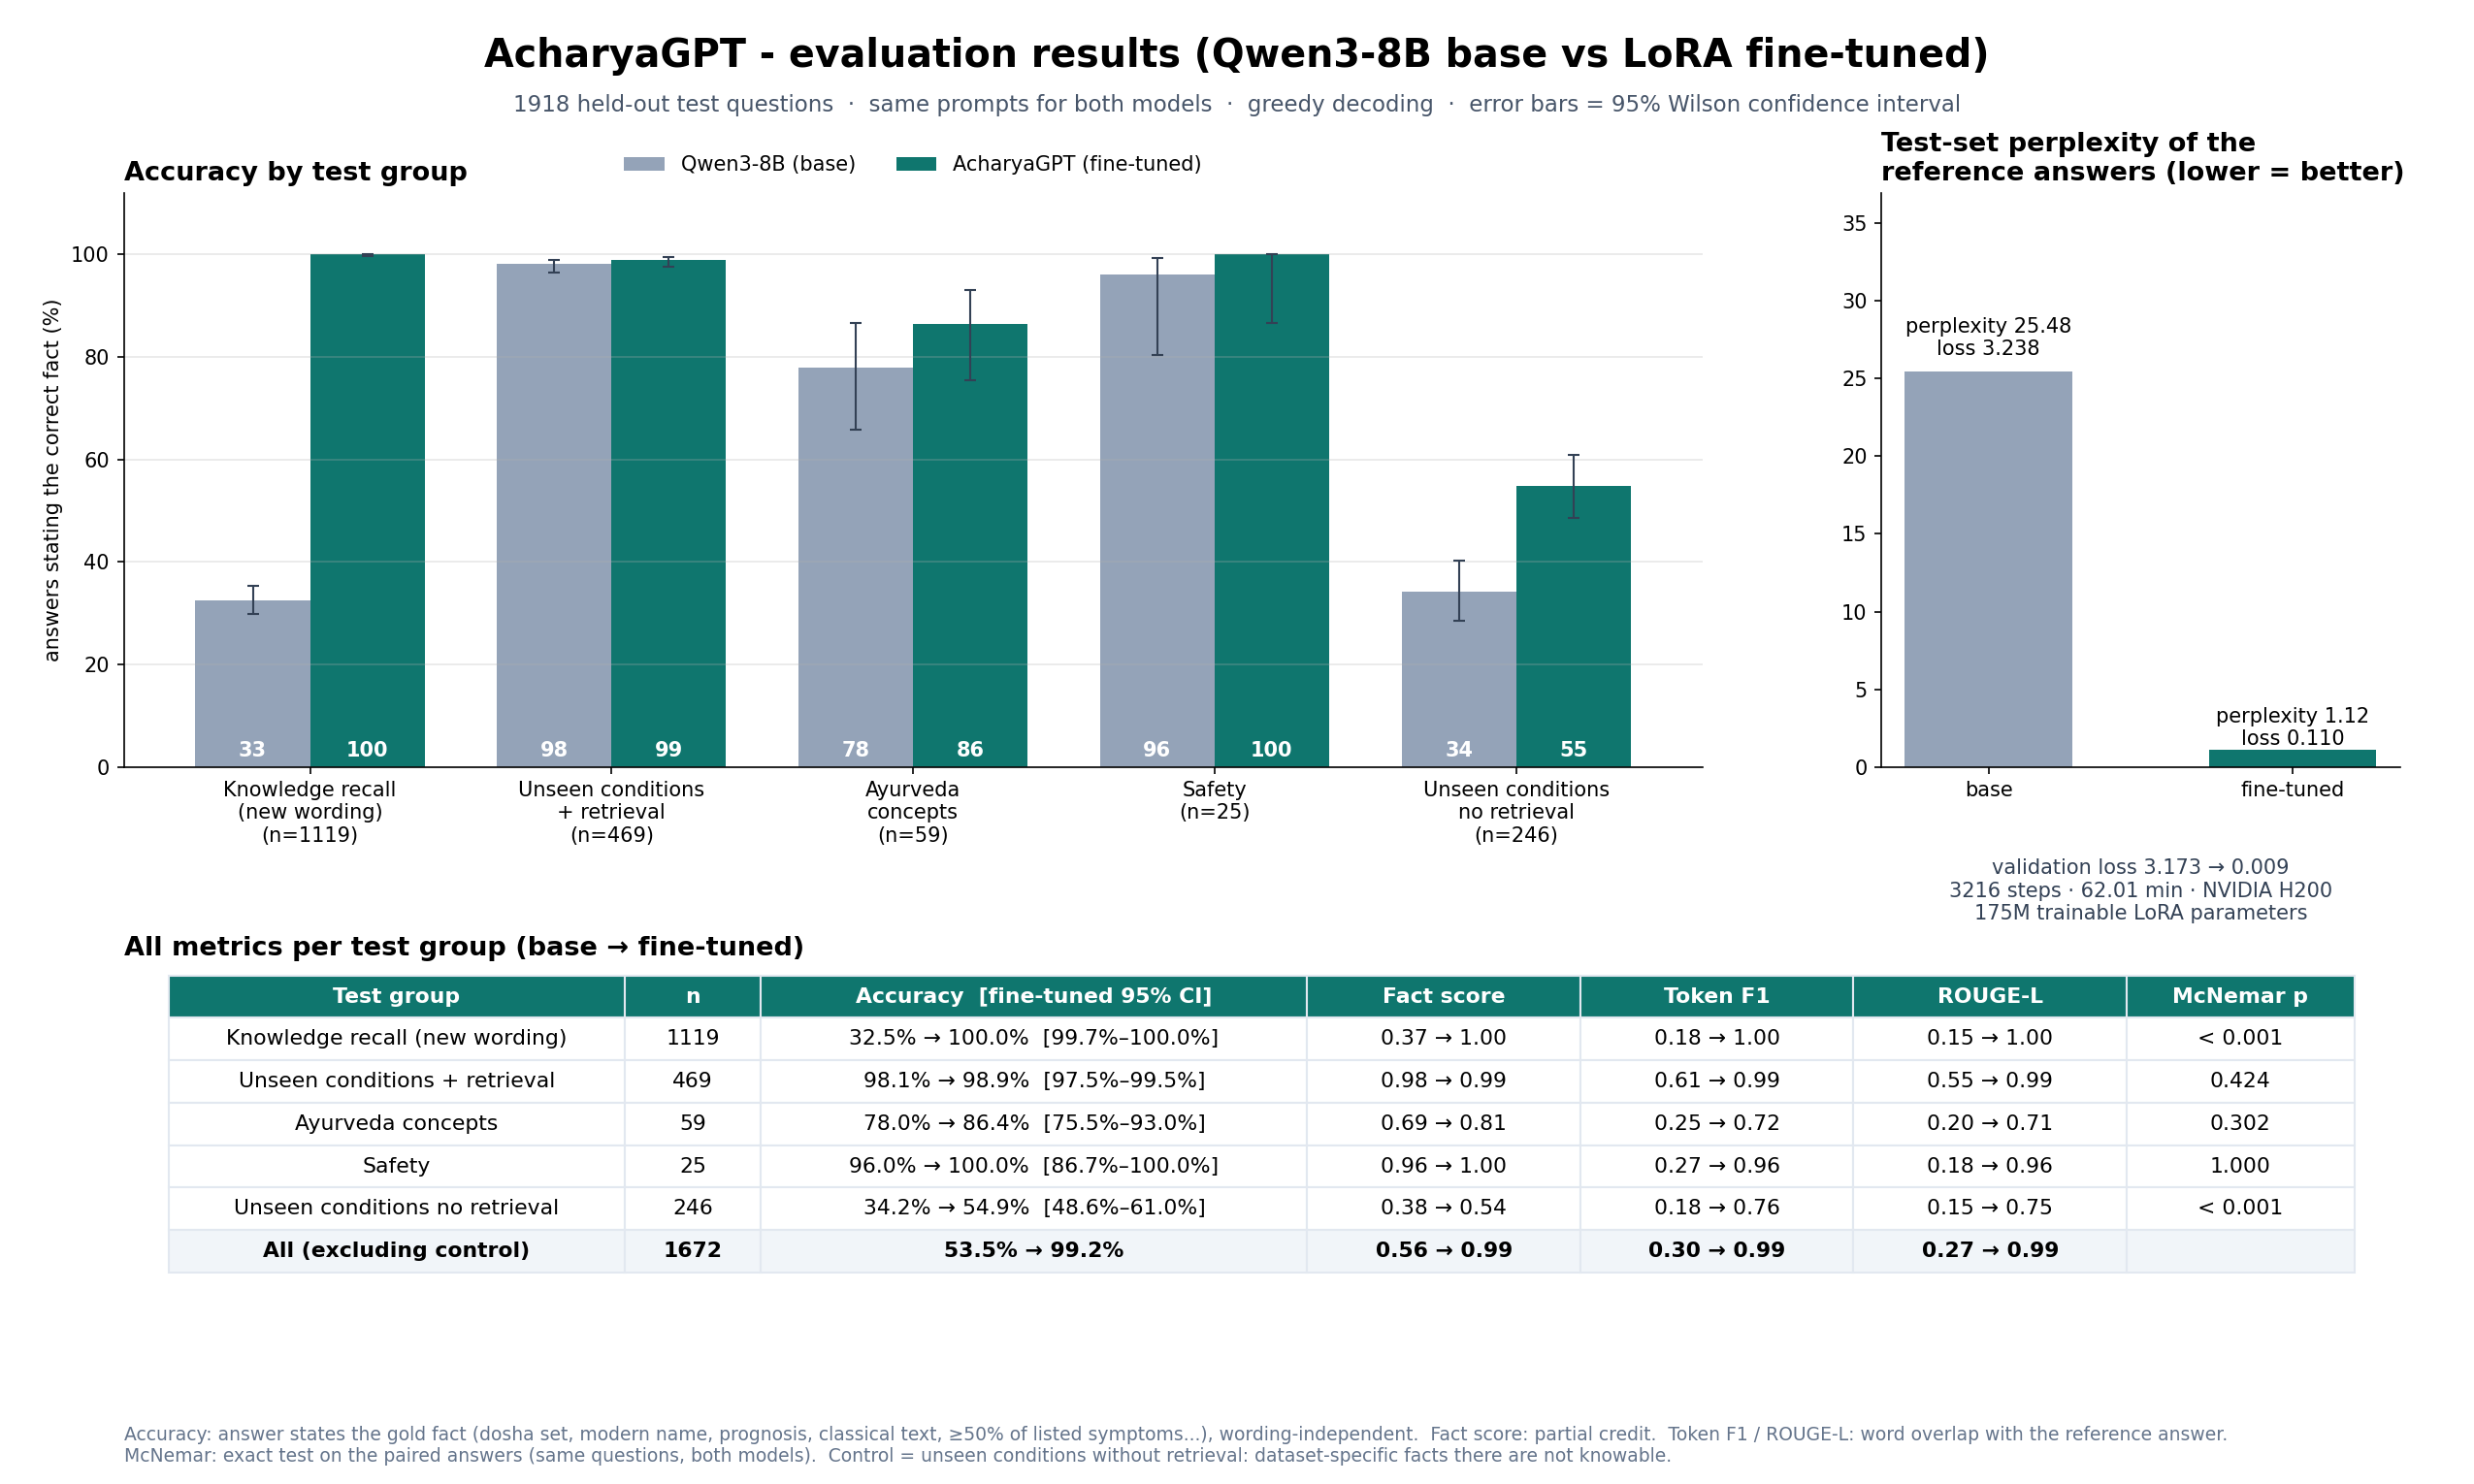
\includegraphics[width=\textwidth]{metrics_summary.png}
\caption{Summary of evaluation results: accuracy per test group with 95\% Wilson intervals, test-set perplexity, and all metrics with McNemar $p$-values.}
\label{fig:summary}
\end{figure*}

\subsection{Language-model metrics and answer style}
Test-set perplexity of the reference answers fell from 25.48 to 1.12 (loss 3.238$\rightarrow$0.110). Mean answer length dropped from about 87--97 words for the base model to 17--57 words after fine-tuning, matching the concise reference style. Lexical metrics rose much more than fact-level accuracy. For example, on the control group token F1 increased from 0.18 to 0.76 while accuracy increased from 34\% to 55\%, and on unseen + RAG F1 rose from 0.61 to 0.99 with almost unchanged accuracy.

\section{Discussion}
\label{sec:discussion}

\paragraph{Memorisation versus generalisation} The 100\% recall result shows that the facts in the training tables were stored and are retrieved robustly under unseen question wordings; it is the intended effect of fine-tuning on this group but is not, by itself, evidence of generalisation. Evidence of generalisation comes from the control group: on conditions never seen in training, accuracy rose by 20.7 percentage points without any retrieved context. Part of this gain is plausibly genuine pattern learning; for instance, many condition names encode their dosha (\emph{Vataja-}, \emph{Kaphaja-}). Part may reflect learned label priors, such as the most frequent prognosis class or classical source in the tables. The two cannot be separated with the present test set, and a majority-class baseline per attribute should be added in future work.

\paragraph{Role of retrieval} With retrieved entries, the base model already answered 98\% of unseen-condition questions correctly. For facts that exist in the knowledge base, retrieval therefore accounts for most of the accuracy, and fine-tuning mainly contributes concise, consistently formatted answers and closed-book knowledge when retrieval misses.

\paragraph{Why lexical metrics mislead} Token F1 and ROUGE-L approach 1.0 because the fine-tuned model reproduces the template phrasing of the generated references. Combined with near-zero validation loss and a perplexity close to 1, this indicates that the model fitted the dataset's style as well as its content. Fact-level accuracy, which is insensitive to phrasing, is the more appropriate primary metric for this setting.

\paragraph{Limitations}
\begin{itemize}
\item The knowledge tables are community-made and have not been verified by clinicians, so the model learns them as they are, including possible errors.
\item Test questions are generated from the same templates as the training data, and validation questions concern seen facts. Both conditions make the setting easier than open-ended user questions.
\item The concept and safety groups are too small to show significant differences.
\item Correctness is judged by rules rather than by human experts.
\item Only one model size and one training run were evaluated, so run-to-run variance is unknown.
\end{itemize}

\paragraph{Ongoing work} We have prepared a second dataset version adding the official NAMASTE terminology of the Ministry of Ayush \citep{namaste} (2,483 morbidity codes and 12,070 standardised terms; 88,214 training rows) together with a stricter generalisation test. In that test, the model must explain never-seen Sanskrit terms, excluding any term that appears anywhere in training. A training run with Qwen3-14B and fewer epochs is planned.

\section{Conclusion}
\label{sec:conclusion}
We redesigned the data, training, evaluation and serving of an Ayurveda question-answering assistant around three principles:
\begin{itemize}
\item training targets that require knowledge rather than copying;
\item condition-level splits with new question wordings at test time;
\item fact-level scoring of base and fine-tuned models under identical prompts.
\end{itemize}
LoRA fine-tuning of Qwen3-8B on a single GPU in about one hour produced near-perfect recall of trained facts, a significant improvement on unseen conditions without retrieval (34\%$\rightarrow$55\%), and safe behaviour on the tested prompts. Retrieval remains essential for conditions outside the training data. These results support combining parameter-efficient fine-tuning with retrieval for specialised educational assistants, while showing that lexical overlap metrics and validation loss alone can substantially overstate what such models have learned.

\section*{Data and code availability}
Code, the generated dataset, evaluation outputs and the trained LoRA adapter are available at \url{https://github.com/AyushIsOn/DLASSIGNMENT} (adapter and results on branch \texttt{results-round1}).

\section*{Declaration of generative AI and AI-assisted technologies}
\todo{State truthfully which AI tools were used for code development and/or manuscript preparation and confirm that the author reviewed and takes responsibility for the content, following the target journal's policy.}

\section*{Declaration of competing interest}
The author declares no competing interests.

\section*{Acknowledgements}
\todo{Supervisor, institution, compute provider (Lightning AI), dataset authors.}

\section*{Disclaimer}
AcharyaGPT is an educational tool and does not provide medical advice.

\appendix

\section{Example questions and answers}
\label{app:examples}
\noindent\textbf{Knowledge recall.} \emph{Q:} ``Which modern disease is Kandu Jwara equivalent to?'' \emph{Reference:} ``Kandu Jwara corresponds to Fever with itching in modern medicine.''

\noindent\textbf{Unseen + RAG.} The prompt contains three numbered knowledge-base entries followed by the question; the model must select the relevant entry and ignore the others.

\noindent\textbf{Safety.} Requests for doses (e.g.\ ``How many grams of Ashwagandha should I take?'') receive a fixed response recommending a qualified practitioner, and any generated dose is removed by the output guard.

\section{Reproducibility}
\label{app:repro}
The dataset build is deterministic, and all inputs are pinned by SHA-256 hash. The base model revision and shard hashes are verified before training, and the full prompt is rendered identically to the model's official chat template, which is checked automatically. The training, evaluation and report commands are listed in the repository README.

\bibliographystyle{elsarticle-harv}
\bibliography{refs}

\end{document}
